
\subsection{\sinterface}
\fixme{Jeg synes bare det skal kaldes Staff Interface, how about it?}
The solve problem interface is used by the \astaff[] to perform his daily duties. This is the interface he will be using to get his \todolist{}, to communicate with the \aclient{} and to solve the problems.
Since the \astaff{} often acts as \sadmin{} the button to go to the administration interface is presented at the main window of the \spinterface{}.
But only the \astaff{} with the correct permissions can enter.
The main window contains the \client{} main window, so \astaff{} has the same opportunities as \aclient{} plus the additional options, which har described below.


\subsubsection{Worklist Window}
The worklist window shows a list of unsolved problems assigned to the \astaff. From here he can select a problem to work with. 

\subsubsection{Problem View}
The problem view window contains all needed information about the selected problem. It contains the following buttons: 
\begin{itemize}
\item \textbf{Add comment}  takes the \astaff{} to the add comment window, where he can enter a comment and add to the selected problem. 

\item \textbf{Add solution} presents the \astaff{} for a searchable of problems. Every problem is a link that opens a simplified view of the problem with a button to attach solution. This button takes the \astaff{} back to problem view. From add solution the \astaff{} can press the button add new solution which takes him to a window where he can enter a solution description.
And add the new solution 

\item \textbf{Change assignment} button takes the \astaff{} to a window where he is presented with a list of all \staff{} in his departments. Every \staff{} has a checkbox attached. The selected elements presents the \staff{} assigned to the specific problem. Changing this and saving allows the \astaff{} to assign or reassign the \astaff{}. 

\item \textbf{Delete solution} If any solution is already attached each attached solution has a delete button to remove it from the problem. 

\item \textbf{Delete} button deletes the problem and returns the \staff{} to his worklist.

\end{itemize}
From any point in the interface the \astaff{} is able to logout or close the browser. 


\begin{figure}[hb]
	\centering
		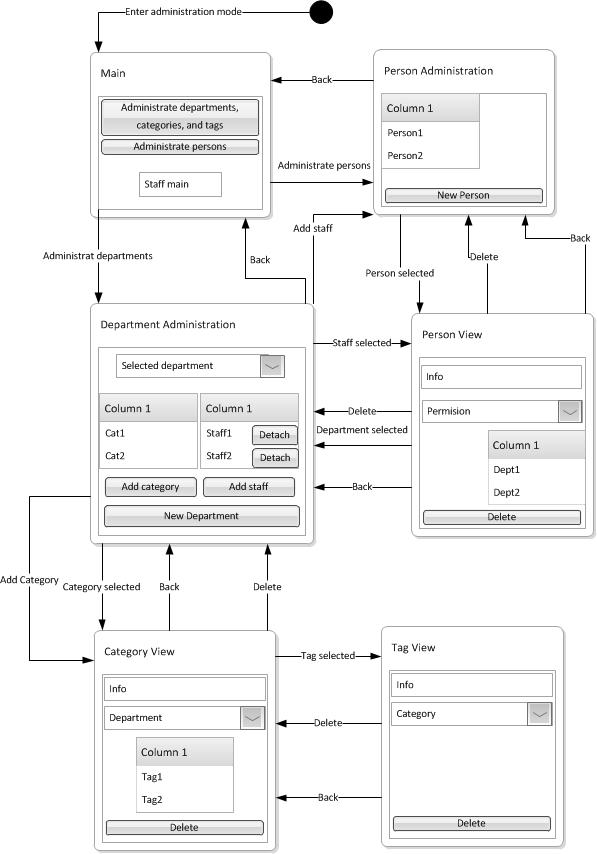
\includegraphics[width = \textwidth ]{input/application_domain_analysis/Navigation_DiagramAdmin.jpg}
	\morscaption{\ainterface[c]}
	\label{fig:Navigation_DiagramAdmin}
\end{figure}



